% Chapter 1 of the Thesis Template File
\chapter{OVERVIEW}

\section{Literate Programming}

The notion of Literate  Programming (LP) [\cite{Knuth:1984:LP:473.479}] provides a potential programming paradigm which brings advantages to software developer. Considering that writing source code need to be seen as an art work, LP handles the input source code by two parts: documentation and implementation. The implementation parts contain the source code in a specific programming language like Java or C/C++. Unlike original programming language (PL) paradigm, the full implementation defined in a LP source file can be split in several parts, which are interleaved by documentation parts. These parts provide descriptions about expected code in natural language. Each documentation parts are corresponded with an implementation part.  A pair of corresponding documentation and implementation part has the same title's prefix.


An example of a LP file, called literate file, is shown in Figure \ref{fig:XStringLPExample}. This file, which is written by C++ published from [\cite{LPExample:XString}]  shows the destructor of the XString class. The implementation part of this method is defined in other area and it is aliased by a documentation part started with "Decrement". The documentation part contains the description of its corresponding code, including what variable needs to be decreed.

\begin{figure}[htp]
	\centering
	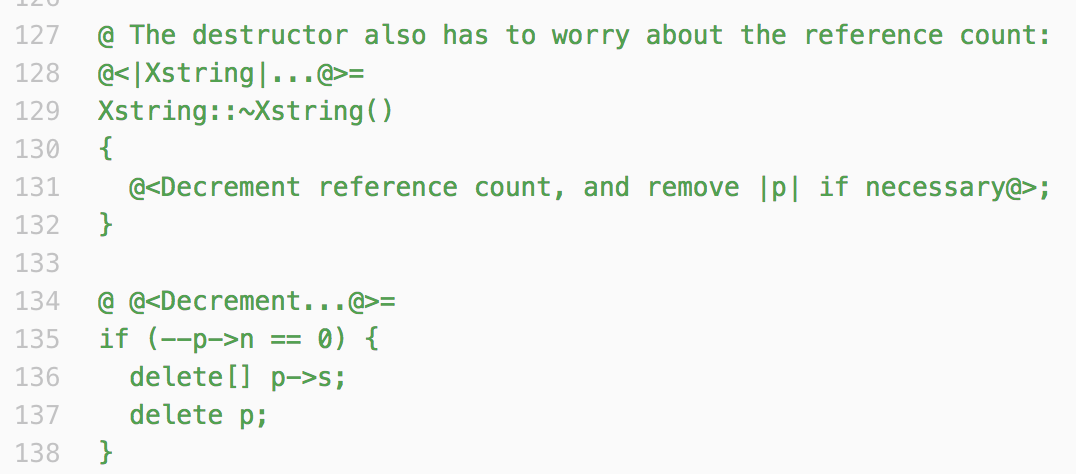
\includegraphics[width=8cm,height=5cm]{resources/fig_lp_file.png}%
	%\includegraphics[width=\textwidth]{conceptdriven.eps}
	\caption[Example of XString.w Literate Programming file in C++]{Example of XString.w Literate Programming file in C++ from [\cite{LPExample:XString}]} 
	\label{fig:XStringLPExample}
\end{figure}

LP provide advantages to software developers. This programming paradigm allows users to understand source code better. It provide a layer to help developers able to read both of natural language (NL) representation and programming language representation of the code. In example showed in Figure  \ref{fig:XStringLPExample}, developers know what action need to do for the destructor in the documentation part, which is decrementing value of a variable, and how to do the action by a decrement assignment and an if statement. Besides, LP helps developer read the documentation parts aligned with the programming parts, which they can check the explanation of behaviors of each program elements instead of reading the implementation and documentation separately. This way of representation make developers be able to imagine about how the source code work for each implementation parts and be able to debug the code easier. In overall, LP provides the more understandable form of source code, including what does the code do and how it works by descriptions in natural language  and descriptions in programming language .

\section{Challenges of realizing Literate Programming}
Realizing LP requires both representation of documentation and implementation parts for each source code file. There are two possible trends to derive these parts, however they faces the problems of effort consuming and low accuracy.
 
\subsection{Manually writing documentation and implementation}
Since the appearance in 1984, LP has not been applied as a popular programming language [\cite{LPArticle:MainStream1}] This fact is surprising since LP provides advantages for code understanding. According to ]cite{}, the main reason is that manually writing the code given documentation parts and manually documented the code given implementation parts are expensive tasks, especially with people who only have background in writing documentation or only have background in writing the code. 

For people who are focusing their work on writing software documentation, doing the implementation part of the documentation are usually infeasible task for them to complete. They know about what elements need to be defined or handled in the implementation and know how program elements involved implementation parts. However, their knowledge is represented by natural language. The most straight forward way for them is learning about programming language to have background of writing code. However, it is not a cheap stacks since it requires 4 years on average for training a Computer Science undergraduate student in the US. Natural Language and Programming Language has many differences how they abstracting the software explanation. For example, in natural language, people can use some indirect reference like pronoun such as "it", "they" while their is no such pronoun representation in some common programming languages like Java. Besides, people who are writing software requirements might need to work with projects in several languages instead of a single programming language, cause it is impossible for them to infer the implementation parts even if they already have background in one language.

From vice versa, people who have experiences in doing the implementation parts of the code might have more background to manually get the documents the code they write. This could be possible and recommended for any developers who are students to do the documents correspond to their small software projects, to make them understand the code better and check the bug in the code faster if bugs exist. However, in industrial projects which contains more than 1000 line of codes, the cost for writing documentation related to each parts of code are expensive, while it can slow down the development process of a software project as half, since developers need to write the explanation for the code they write. In addition, the code does not stay the same and code are updated days by days following requirements of users. This fact brought challenges for software developers to manually write documentation although they have good background for explaining the code in natural language. In overall, manually writing both documentation parts and implementation  are expensive. So that, approach for automatically deriving documentation and implementation are important.

\subsection{Automatically  inferring implementation by Machine Translation }
 In translation between natural languages, phrase based machine translation (PBMT) and Neural Machine Translation (NMT) are two common machine translation (MT) approaches that show their effectiveness for the inference problems. This fact brings MT as the most used translation engines [\cite{8416973}]. We might think about a solution for the software engineering is that applying MT to inferring implementation from documentation, given the intuition that both implementation and documentation have the same intension of describing how computer program works. However, researches on using MT in this area still not have good results yet [\cite{DBLP:journals/corr/BaroneS17}], due to several following problems.
\subsubsection{Lack of high quality Parallel corpus}
In natural language processing, current MT techniques rely on large scale corpus, which contains 10000 to millions pairs between different languages \cite{}. Machine learning algorithms like Bayesian learning are used to learn the mapping between source and target  languages. The corpus needed to be prepared as pairs of sentences, and the target languages need to be written manually by linguistic experts. However, in software engineering, building such a parallel corpus for documentation and implementation manually are expensive. 
Another approach is to relying on documentation written as natural language code comments. This seems to be a good direction since large scale code corpus contains millions line of code (LOC) and there are textual description in the form of code comments for each source code files. However, this type of documentation doesn't guarantee to have the same intent of describing the behavior of related source code. For example. this documentation contains "TODO" tags which are automatically generated by the IDE, or  contains comments that are actually source code which is commented by developers. In fact, such a corpus generated by documentation in the form of code comments and implementation contains noise and cause very low quality inference in MT models \cite{} .
Along with the problems from the shortage of good parallel corpus, MT also facing the problems from the differences between natural language and programming language, A survey \cite{} summarized the main differences between two languages which hindered an MT models for learning mapping between two languages. In general, it comes from the different purpose of translation between natural language processing and program generation, and more important, natural language and programming language have different mechanism of indirect reference management \cite{}.
\subsubsection{MT for Natural Language to Natural Language: Descriptive Model}
In Natural Language, the main purpose for inferring the target language is to helping user understand about the main idea of the source sentence. In the other words, it solved like providing the description for the content of source language, which include what is the main subject, what are the verbs and what are objects used in the sentence in a form of a sample subject-verb-object structure sentence. Let's see an example in figure \cite{}. In this example, which I observed from NMT system for Germany to English translation published by tensorflow \cite{}, the generated neural machine translation result shows almost the same with the expected sentence except one word "Halef" which is a last name. From this generated sentence, users can easily understand the meaning of the sentence and this kind of missing words error are acceptable. In NL, MT worked as a descriptive model, which allows thhe translated result missed one or two words compared to the expected sentence while users still understand.
\subsubsection{MT for Natural Language to Programming Language: Generative Model}
In contrast with NL-to-NL translation, the direction of natural language to programming language requires a very precise generated result. We can look at an example in figure \cite{}. SpecTrans \cite{} is a statistical machine translation system for inferring between documentation and implementation for java specification. The phase of inferring implementation returns 27 \% of syntactically correct. SpecTrans returns 38 \% of results are close to the expected result like this example. In the example in \cite{}, although we only used two edit actions to get the correct result, the translated implementation are still syntactically incorrect and cannot use directly as an generated source code. The problem of syntactically incorrect doesn't appear only in documentation to implementation translation but also in translating between object oriented programming languages. SemSMT \cite{} shows that there are over 60\% of translated results are syntactically incorrect. In overall, generating code from source, even if documentation or code from other programming language is an error-prone task by machine translation.
\subsubsection{Differences in indirect references between Natural Language and Programming Language}
\cite{} summarized problems of the generation of code from natural language of several existing tools. In general, the most important is that they have unique ways for handling indirect references. An example of such types of differences is shown by example \cite{}. In this example, a variable x can be described by the pronoun "it" in natural language as an indirect reference to variable x. However, in the implementation, there is only one way for represent variable x. These differences brings challenges for MT system to learn the mapping between languages. We will describe about types of indirect references between natural language and programming language in the next section.


\section{Direction of  a syntax-based approach for Natural Language to Programming Language translation}
Realizing Literate Programming can take benefits from a module for automatically generating code from documentation. However, the building of such a module based on machine translation engines used in natural language processing faced challenges. In this project, we analyze the problem from another aspect instead of relying on statistical approach. Our intuition is that, natural language description can be represented as a natural language parser by \cite{}, and each type of nodes in the parsed tree has rules for the translation by a syntax-based approach. To achieve this task, we conduct my research in the following steps.  First, according to survey \cite{}, we studied main problems of indirect references between two languages. Next, we studied each node types in Natural Language parser and propose rules for translation. After that, we implement a module that embedded these rules in an Natural Language Visitor based on the idea of ASTVisitor in programming language, to translate the code comment for each source files of a java project. We build a tool as an online IDE for users to do literate programming and publish on the site \cite{}. 









